\section{Finite-element formulation and verification}
\label{sec:fem}

This section specifies the finite-element method for the coupled problem of Section~\ref{sec:formulation},
states what has and has not been verified, and reports the verification of the wall idealisation.
\textbf{The coupled fluid--structure--thermal solver is specified here but no result of it is reported.}
The only finite-element computations in this paper are those of the wall in
Section~\ref{sec:q8}.

\subsection{Discretisation}
\label{sec:fe}
\emph{Meshes.} The fluid and the solid are meshed separately but conformingly: the two meshes share the
nodes of $\Ga_{\mathrm{if}}$, so that interface data need no interpolation. The fluid mesh follows the
deformed interface through the extension problem of Section~\ref{sec:ale}.

\emph{Fluid.} Velocity and pressure use the Taylor--Hood pair, continuous quadratic velocity and
continuous linear pressure (P2--P1), which satisfies the discrete inf--sup condition
\citep{hood1974navier,brezzi1991mixed}. On $\Om_f$ the weak form seeks $(\bu,p)$ with $\bu$ satisfying B1
and B3--B4 and the interface condition $\bu=\bm0$ such that, for all admissible $(\bv,q)$,
\begin{equation}
\int_{\Om_f}\!\left[\rho(\bu\!\cdot\!\nabla\bu)\!\cdot\!\bv+2\mu\,\bD(\bu)\!:\!\bD(\bv)-p\,\nabla\!\cdot\!\bv+q\,\nabla\!\cdot\!\bu\right]\dd\Om=0,
\label{eq:wkfluid}
\end{equation}
where the do-nothing outflow B2 is the natural condition. The convective term is linearised by Newton
iteration.

\emph{Energy.} Temperature is one continuous quadratic field $T$ on $\Om_f\cup\Om_s$ with the
conductivity $k=k_f$ or $k_s$ and the velocity $\bu$ in the fluid and zero in the solid. Because the
meshes are conforming, temperature continuity \eqref{eq:iftemp} is enforced strongly and the flux
continuity \eqref{eq:ifflux} is the natural interface condition: there is a \emph{single} interface
temperature unknown and no thermal interface iteration. With B5 the weak form is
\begin{equation}
\int_{\Om_f\cup\Om_s}\!\left[\rho c_p(\bu\!\cdot\!\nabla T)\,\phi+k\,\nabla T\!\cdot\!\nabla\phi\right]\dd\Om
+\sum_K\int_K\tau_K\,\rho c_p\,\bu\!\cdot\!\nabla\phi\,\mathcal R_K(T)\,\dd\Om=\int_{\Ga_h}\qpp\,\phi\,\dd\Ga,
\label{eq:wkenergy}
\end{equation}
with the element residual $\mathcal R_K(T)=\rho c_p\,\bu\!\cdot\!\nabla T-k_f\nabla^2T$. The
streamline-upwind/Petrov--Galerkin (SUPG) term \citep{brooks1982streamline} is required: the P\'eclet number is
$\mathrm{Pe}=\NumPe$, so that a Galerkin discretisation without stabilisation is expected to oscillate on any mesh whose
streamwise spacing is not of micrometre order. The stabilisation parameter is
$\tau_K=\tfrac{h_K}{2|\bu|_K}\left(\coth\mathrm{Pe}_K-1/\mathrm{Pe}_K\right)$ with
$\mathrm{Pe}_K=\rho c_p|\bu|_Kh_K/(2k_f)$ and $\tau_K=0$ in the solid.

\emph{Solid.} The displacement is continuous quadratic. To retain the beam--column amplification of
Section~\ref{sec:beamcolumn} the solid is solved in a total-Lagrangian description with the
Green--Lagrange strain $\bm E=\tfrac12(\bm F^{\mathsf T}\bm F-\bm I)$, the deformation gradient
$\bm F=\bm I+\nabla\bd$, and the St~Venant--Kirchhoff law with the in-plane thermal eigenstrain of A1,
\begin{equation}
\bm S=\mathbb C\!:\!\left[\bm E-(1+\nu)\alpha\,\theta\,\bm I\right],\qquad
\int_{\Om_s^0}\bm S\!:\!\delta\bm E\,\dd\Om=\int_{\Ga_{\mathrm{if}}^0}\bm t\!\cdot\!\delta\bd\,\dd\Ga,
\label{eq:wksolid}
\end{equation}
where, for small strain and rotation, \eqref{eq:wksolid} reduces to the linear system \eqref{eq:solid}, and $\theta=T_s-T_{\mathrm{in}}$ is the temperature rise and $\bm t$ is the fluid traction pulled back to
the reference interface. The tangent of \eqref{eq:wksolid} contains a material part and a geometric part
that carries the thermal membrane stress; the latter is what produces the amplification
$1/(1-N_c/\ncr)$. A linear solid omits it (Section~\ref{sec:q8nl}).

\subsection{Coupled fixed-point algorithm}
\label{sec:algorithm}
The mechanical coupling is a Dirichlet--Neumann partition: the fluid receives the interface displacement
through the mesh extension, and the solid receives the interface traction. With the thermal problem
solved as one field, the outer iteration $k=0,1,\dots$ on the deformed geometry
$\Om^k$ ($\Om^0$ undeformed) is:
\begin{enumerate}
\item solve the Navier--Stokes problem \eqref{eq:wkfluid} on $\Om_f^k$ for $(\bu^k,p^k)$ and form the
interface traction $\bm t^k$;
\item solve the energy problem \eqref{eq:wkenergy} on $\Om_f^k\cup\Om_s^k$ for $T^k$, hence $\theta^k$ in the solid;
\item solve \eqref{eq:wksolid} with $\theta^k$ and $\bm t^k$ for $\bd^{k+1}$;
\item relax, $\bd^{k+1}\leftarrow\omega\bd^{k+1}+(1-\omega)\bd^k$ with $0<\omega\le1$ (Aitken updating is optional), and
update the fluid mesh through the extension problem of Section~\ref{sec:ale};
\item stop when $\|\bd^{k+1}-\bd^k\|/\|\bd^{k+1}\|$ and the relative interface heat-flux imbalance are below tolerances.
\end{enumerate}
The guards of Section~\ref{sec:guards} are monitored during the iteration; in particular the
mesh-quality guard G1 keeps the extension problem well posed. A partitioned thermal alternative, in which
the interface temperature is imposed as a Dirichlet condition on the solid and the flux as a Neumann
condition on the fluid, is possible on the same meshes but is not needed here. \emph{No proof of convergence
of the fixed point is offered.} The reduced-order estimates of Section~\ref{sec:indicative} indicate a weak
return coupling at the baseline, which suggests contraction, but this has not been tested.

\subsection{Verification hierarchy}
\label{sec:hier}
Table~\ref{tab:hier} lists the verification levels needed before coupled results could be trusted and
shows which have been executed. Only the first four concern the wall and the reduced-order model; all
levels involving the fluid are planned.

\begin{table}[t]
\centering\small
\caption{Verification hierarchy. ``Done'' marks computations reported in this paper.}
\label{tab:hier}
\begin{tabular}{@{}p{0.8cm}p{6.4cm}p{4.6cm}p{1.3cm}@{}}
\toprule
Level & Test & Reference & Status \\
\midrule
V1 & Shape functions, patch test (Q8) & exact polynomial field & Done \\
V2 & Closed forms of Section~\ref{sec:reduced} against an independent boundary-value solution & analytic/numerical BVP & Done \\
V3 & Free bow of the wall, end supports, mesh study & $\kth L^2/8$ & Done \\
V4 & Restrained nonlinear wall, amplification and membrane force; independent code; thin-strip limit & beam--column & Done \\
V5 & Rigid slit, pressure drop and velocity profile & $12\mu UL/H_0^2$ (Poiseuille) & Planned \\
V6 & Rigid slit, one wall heated, developed Nusselt number & \citet{shah1978laminar} & Planned \\
V7 & Conjugate transfer with a rigid thick wall & \citet{rahimi2024conjugate} & Planned \\
V8 & Pressure-loaded compliant channel, flow rate--pressure drop & \citet{christov2018flow} & Planned \\
V9 & Mesh convergence of the coupled outputs ($w$, $\Delta p$, $\mathrm{Nu}$) & \citet{celik2008procedure} & Planned \\
V10 & Iteration history and interface energy balance of the fixed point & internal consistency & Planned \\
\bottomrule
\end{tabular}
\end{table}

\subsection{Verification of the wall idealisation}
\label{sec:q8}
Two plane-strain computations with eight-node serendipity (Q8) elements, $3\times3$ Gauss quadrature and
a sparse direct solver, are reported. Both are own implementations (\texttt{code/q8\_strip.py} and
\texttt{code/q8\_nonlinear.py}); the second is cross-checked with an independent code in Section~\ref{sec:slender}. The shape functions are checked for partition of unity and for their
derivatives against central differences, and the patch test (the exact stress-free thermal-bending field must
satisfy the discrete equations) is passed on every mesh with a maximum relative residual of
$\QPatchMax$.

\subsubsection{Free bow and end supports}
\label{sec:q8free}
With a linear through-thickness temperature of zero mean the beam theory gives the bow
$w=\kth L^2/8$ at mid-span (Section~\ref{sec:freecurv}). The finite-element value is sampled at the
\emph{fixed} physical point $(L/2,\,y=d/2)$ on every mesh, because a sampling height that changes with the
through-thickness refinement is not a property of the mesh. Three end idealisations are compared:
an ideal point pin ($u_y=0$ at the single mid-surface node of each end edge), the pin of the paper realised
as $u_y=0$ on the whole end edge, and a clamp ($u_x=u_y=0$ on the whole edge). Meshes range from $6\times2$ to
$192\times8$ elements ($N_x\times N_y$, at most \QElemMax{} elements); the results are normalised by
$\kth L^2/8$ and are in Table~\ref{tab:q8mesh} and Figure~\ref{fig:q8mesh}.

\begin{table}[t]
\centering\scriptsize
\caption{Free-bow study: mid-span, mid-surface deflection normalised by $\kth L^2/8$. The order $p$,
the extrapolated value and the grid-convergence index (GCI, safety factor 1.25) of the clamp are from the
last three axial refinements, $N_x=48,96,192$ \citep{celik2008procedure}.}
\label{tab:q8mesh}
% AUTO-GENERATED by make_numbers.py
\begin{tabular}{@{}rrcccccrr@{}}
\toprule
$N_y$ & elements & point pin & full-edge pin & clamp & clamp & $p$ & clamp, extrap. & GCI (\%) \\
 & ($N_x=192$) & ($N_x=192$) & ($N_x=192$) & ($N_x=24$) & ($N_x=192$) & & & \\
\midrule
2 & 384 & 1.00000 & 0.99793 & $-$0.0288 & $-$0.0195 & 1.7 & $-$0.0192 & 2.0 \\
4 & 768 & 1.00000 & 0.99800 & $-$0.0253 & $-$0.0180 & 1.3 & $-$0.0175 & 3.8 \\
8 & 1536 & 1.00000 & 0.99800 & $-$0.0238 & $-$0.0174 & 1.1 & $-$0.0168 & 4.2 \\
\bottomrule
\end{tabular}

\end{table}

\begin{figure}[t]
\centering
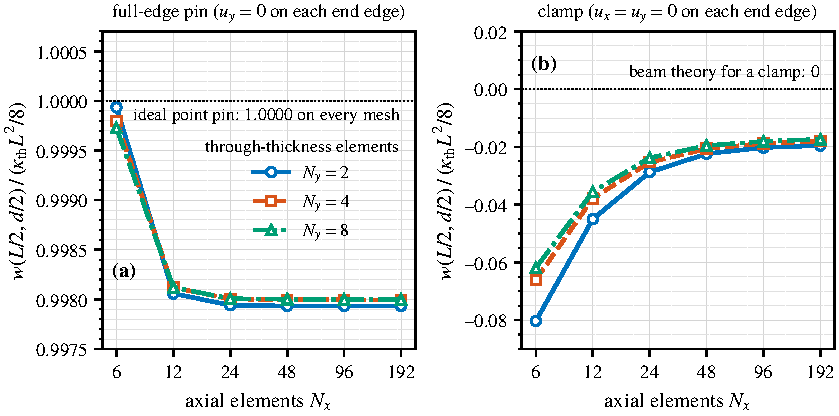
\includegraphics[width=\textwidth]{figures/fig4_q8_mesh.pdf}
\caption{Free-bow study against axial refinement $N_x$ for $N_y=2,4,8$ elements through the thickness.
(a) Pin realised as $u_y=0$ on each end edge. (b) Clamp.}
\label{fig:q8mesh}
\end{figure}

The ideal point pin returns $\QPointMin$ on every mesh, as it must: the exact field lies in the element
space, so this result tests the implementation and not the convergence. The pin of the paper, $u_y=0$ on the
whole edge, gives $\QPinFour$ at $192\times4$ and $\QPinEight$ at $192\times8$, a defect of
$\QPinDefect\,\%$. This is mesh-independent: the value changes by $\QPinAxialLast$ between $N_x=96$ and
$192$ at $N_y=8$ and by $\QPinThickLast$ between $N_y=4$ and $8$ at $N_x=192$. The defect is therefore a property of the
end condition and not a discretisation error. The clamp bows slightly \emph{towards} the channel. Beam theory
gives zero, since a clamp forbids end rotation and a uniform-curvature strip then does not bow; the
finite-element value converges slowly to a small negative number (Table~\ref{tab:q8mesh},
extrapolated $\QClampInfEight$ at $N_y=8$). The observed order is below two ($p=\QClampOrderEight$ at $N_y=8$), so the
asymptotic range has not been established and the GCI of $\QClampGCIEight\,\%$ is indicative only. The relevant
conclusions are that the pin idealisation is reproduced to $\QPinDefect\,\%$ and that the clamp, which is not
used in this paper, reduces the bow to $\QClampLastEight$ times the pinned bow, in agreement with beam theory (zero)
to that level.

\subsubsection{Restrained, geometrically nonlinear wall}
\label{sec:q8nl}
The baseline wall is not free: its ends are restrained axially (A7, B6), and the mean temperature rise
$\bar\theta=\NLthetaBar$~K produces the compressive membrane force $N_c$ of Section~\ref{sec:buckling}. The
second computation solves this problem: $\theta(Y)=\bar\theta+\Delta T_t(Y/d-\tfrac12)$ with the values of
Table~\ref{tab:baseline}, $u_y=0$ on the end edges, and a linear constraint that makes the mean axial displacement of each
end edge zero, eliminated exactly. The solid is the total-Lagrangian model \eqref{eq:wksolid} without
fluid load, solved by Newton iteration in four thermal load steps. The analytic tangent agrees with a central
finite difference of the residual to $\NLtangentMax$, and every step converged in at most $\NLnewtonMax$
iterations to a relative residual of $\NLresMax$. The same data are solved with the linear solid (material stiffness only)
for comparison; Table~\ref{tab:q8nl} and Figure~\ref{fig:q8nl} show the results.

\begin{table}[t]
\centering\small
\caption{Restrained wall at the baseline: linear and nonlinear Q8 solutions. $w^{\mathrm{lin}}$ is the
linear-solid mid-span deflection; $w_{\max}^{\mathrm{NL}}$ the total-Lagrangian one; $N_c$ is the
membrane force in the two element columns adjacent to mid-span.}
\label{tab:q8nl}
% AUTO-GENERATED by make_numbers.py
\begin{tabular}{@{}lrcccc@{}}
\toprule
mesh $N_x\times N_y$ & elements & $w^{\rm lin}/(\kth L^2/8)$ & $w_{\max}^{\rm NL}$ (\si{\micro\metre}) & $w_{\max}^{\rm NL}/H_0$ & $N_c$ at mid-span (kN\,m$^{-1}$) \\
\midrule
$24\times2$ & 48 & 0.9979 & 223.39 & 0.4468 & 27.79 \\
$48\times4$ & 192 & 0.9980 & 222.46 & 0.4449 & 27.74 \\
$96\times4$ & 384 & 0.9980 & 222.33 & 0.4447 & 27.74 \\
$96\times8$ & 768 & 0.9980 & 222.17 & 0.4443 & 27.73 \\
$192\times8$ & 1536 & 0.9980 & 222.14 & 0.4443 & 27.73 \\
\bottomrule
\end{tabular}

\end{table}

\begin{figure}[t]
\centering
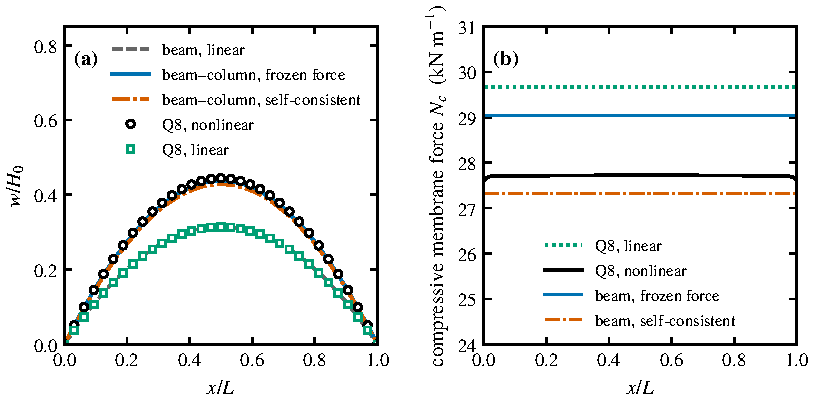
\includegraphics[width=\textwidth]{figures/fig5_q8_nonlinear.pdf}
\caption{Restrained baseline wall, finest mesh ($192\times8$). (a) Mid-surface deflection. (b) Compressive membrane
force per element column. Beam values are those of Table~\ref{tab:baseline}.}
\label{fig:q8nl}
\end{figure}

The results are as follows. (i) The linear-solid bow is $\NLlinRatio\,\kth L^2/8$, equal to the full-edge pin value of
Section~\ref{sec:q8free}: in a linear solid the membrane force does not couple to the bending. (ii) The
linear solution carries the membrane force $\NLNmidLin$~kN\,m$^{-1}$ at mid-span, $\NLNmidLinPct\,\%$ above the
frozen-force beam value of Table~\ref{tab:baseline}. (iii) The nonlinear solid bows by
$\NLwFE$~m ($\NLwFEH\,H_0$), an amplification $\NLampFE$ over the linear value, compared with $\NumAmpFrozen$
(frozen force) and $\NumAmpSc$ (self-consistent) in the beam--column model. A linear finite-element solid
therefore under-predicts the bow by a factor $\NLampFE$, which is why the total-Lagrangian form is specified in
Section~\ref{sec:fe}. (iv) The membrane force relaxes from $\NLNmidLin$ to $\NLNmidNL$~kN\,m$^{-1}$, that is by
$\NLrelaxFE\,\%$, against $\NumRelax\,\%$ in the beam model: the arc-stretching relaxation of
Section~\ref{sec:beamcolumn} is reproduced in magnitude. (v) The finite-element deflection exceeds the
self-consistent beam--column value by $\NLoverScPct\,\%$ and the frozen-force value by $\NLoverFrozenPct\,\%$.
(vi) The nonlinear result changes by $\NLconvAxial\,\%$ between $N_x=96$ and $192$ and by $\NLconvThick\,\%$ between
$N_y=4$ and $8$, so it is mesh-converged at this level.

\subsubsection{Independent solution and the thin-strip limit}
\label{sec:slender}
\emph{Independent code.} The same boundary-value problem was solved with a different code base and discretisation:
scikit-fem, six-node quadratic triangles, Lagrange-multiplier constraints for the end conditions, a different mesh
(\IndElements{} triangles at the finest level) and different quadrature (\texttt{code/fe\_independent.py}). It gives
$\IndW$~m for the nonlinear bow, which differs from the Q8 value by $\IndDiffPct\,\%$, and the mid-span membrane force
differs by $\IndNDiffPct\,\%$; the linear solutions agree to within $10^{-4}\,\%$. The result of the triangle mesh
itself changes by $\IndConv\,\%$ between the last two refinements. The two codes share the equations
(St~Venant--Kirchhoff kinematics, eigenstrain model), so this agreement verifies the implementation and the
discretisation but not the modelling assumptions.

\emph{Is the departure from the beam model a thickness effect?} Beam theory contains neither shear flexibility nor
end effects, so if the $\NLoverScPct\,\%$ of item (v) were due to the thickness of the strip ($d/L=0.1$) it must
vanish as $d/L\to0$ at fixed dimensionless loading. The study of Table~\ref{tab:slender} keeps the free curvature and the
force ratio $N_c/\ncr=\SlForceRatio$ fixed (so $\bar\theta\propto d^2$ and $\Delta T_t\propto d$) and varies $d$ with the
independent code. The departure from the self-consistent beam--column value falls from $\SlFirstPct\,\%$ at $d/L=0.1$ to
$\SlMidPct\,\%$ at $d/L=\SlMidDL$ and $\SlLastPct\,\%$ at $d/L=\SlLastDL$, roughly as $(d/L)^2$, and the
finite-element membrane force tends to the self-consistent beam force. At $d/L=\SlLastDL$ the result changes by only $\SlMeshPct\,\%$ between the $192\times8$ and $384\times16$ meshes, so the
residual of $\SlLastPct\,\%$ is not a mesh error. It is of the size expected of the higher-order rotation terms that the
von K\'arm\'an beam--column model omits (the maximum slope is $\NumSlope$), but this was not isolated. The departure of the baseline is therefore a finite-thickness effect of the
two-dimensional wall, and not a disagreement between the equations of the beam model and those of the finite-element
model. The finite-element value, in contrast, lies $\SlLastFrozenPct\,\%$ below the frozen-force value at $d/L=\SlLastDL$: its proximity to the baseline
finite-element result ($\NLoverFrozenPct\,\%$) is a coincidence of thickness, not an accuracy property.

\begin{table}[t]
\centering\small
\caption{Thin-strip study with the independent code: curvature $\kth=\NumKappa$~m$^{-1}$ and $N_c/\ncr=\SlForceRatio$ held
fixed, mesh $192\times8$. Columns: linear bow relative to $\kth L^2/8$, nonlinear bow relative to the self-consistent (sc)
and frozen-force (ff) beam--column values, and membrane force relative to the self-consistent beam force.}
\label{tab:slender}
% AUTO-GENERATED by make_numbers.py
\begin{tabular}{@{}cccccc@{}}
\toprule
$d/L$ & $d$ (mm) & $w^{\rm lin}_{\rm FE}/w^{\rm lin}_{\rm beam}$ & $w^{\rm NL}_{\rm FE}/w_{\rm sc}$ & $w^{\rm NL}_{\rm FE}/w_{\rm ff}$ & $N_{c,\rm FE}/N_c^{\rm sc}$ \\
\midrule
0.100 & 3.00 & 0.9980 & 1.0383 & 1.0152 & 1.0146 \\
0.075 & 2.25 & 0.9989 & 1.0233 & 0.9846 & 1.0083 \\
0.050 & 1.50 & 0.9995 & 1.0092 & 0.9330 & 1.0021 \\
0.035 & 1.05 & 0.9998 & 1.0017 & 0.8720 & 0.9993 \\
0.025 & 0.75 & 0.9999 & 0.9976 & 0.7990 & 1.0010 \\
\bottomrule
\end{tabular}

\end{table}

For the baseline strip the reduced-order deflection of Section~\ref{sec:baseline} is therefore a slight under-estimate,
by $\NLoverScPct\,\%$, of the two-dimensional wall response. For design use the finite-element value
$\NLwFEH\,H_0$ should be preferred for this thickness; the guard values and ceiling heat fluxes derived from the
reduced-order model are correspondingly slightly non-conservative.

\subsection{What has been verified}
The reduced-order model of the wall is verified against an independent boundary-value solution (V2) and, in
two dimensions, against finite elements (two independent codes) for the free bow, the end condition, the membrane force and the
nonlinear amplification, including the limit of a slender strip (V1, V3, V4). The constitutive and kinematic assumptions common to all
the wall models are not independently validated against experiment. The fluid-side estimates of Section~\ref{sec:indicative}, the coupling
algorithm and the formulation of the interface remain unverified until V5--V10 are carried out.
